\documentclass{article}

% Pour utiliser toues les fonctions du clavier
\usepackage[utf8]{inputenc} % un package
\usepackage[T1]{fontenc}      % un second package

% Choix de la langue
\usepackage[francais]{babel}  % un troisième package
\setlength{\parindent}{0pt}

% Taille des marges
\usepackage[top=2.5cm, bottom=2cm, left=2.5cm, right=1.5cm]{geometry}

% Pour l'espace entre les lignes
\usepackage{setspace}
% Utilisation:
% Moyen:
% \begin{onehalfspace}
% \end{onehalfspace}
% Grand:
% \begin{doublespace}
% \end{doublespace}

% Changement des polices
\usepackage{charter}

% Pour afficher du code
\usepackage{verbatim}
\usepackage{moreverb}


\usepackage{titling}
\setlength{\droptitle}{-5em}   % This is your set screw

% Version 2
\usepackage{listings}

% Couleurs
\usepackage{color}
\usepackage[dvipsnames]{xcolor}
\usepackage{colortbl}

\title{Rapport Labo 3}
\author{Lucas \bsc{Bulloni} \&Bastien \bsc{Wermeille}}
%\date{10 Novembre 2017}

% En-têtes et pieds de pages
\usepackage{fancyhdr}
 
\pagestyle{fancy}
\fancyhf{}
\rhead{Lucas \bsc{Bulloni} \&Bastien \bsc{Wermeille}}
\lhead{Réseau et application}
\chead{Rapport Labo 2}
\cfoot{\thepage}

% Package pour la légende de la table
\usepackage{caption}

% Package de multi-colonnes
\usepackage{multicol}

% Package pour les images
\usepackage{graphicx}

%bibliographie
\usepackage{biblatex}
\addbibresource{biblio.bib}{}

% Pour les listes
\usepackage{enumitem}
\setlist[itemize]{topsep=0pt,after=\newline}

% package pour liens hypertexte
\usepackage{hyperref}

%\usepackage{minted}

% Début du document
\begin{document}

\maketitle

 

\section{Introduction}
 Le but de ce travail pratique est la découverte de techniques permettant de réaliser de la "Quality of Service" (QoS) sur un réseau simple. Ainsi que de tester ces dernières dans un environnement Netkit.

\subsection{Matériel à disposition}
\begin{enumerate}
\item 1 Linux PC with NetKit
\item Laboratoir netkit "qos"
\end{enumerate}

\section{Méthodologie}


\subsection{Cas concret}
Grace au fichier lab.conf, nous pouvons déterminer la structure du réseau étant celle-ci:
\begin{figure}
  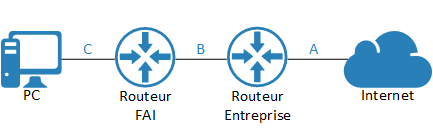
\includegraphics[width=\linewidth]{./Structure.png}
  \caption{Démarrage du labo netkit "QoS"}
  \label{fig:qos}
\end{figure}

Figure \ref{fig:qos} représente le démarrage du laboratoir netkit "qos".


Démarrage du laboratoir NetKit "qos":
\begin{figure}
  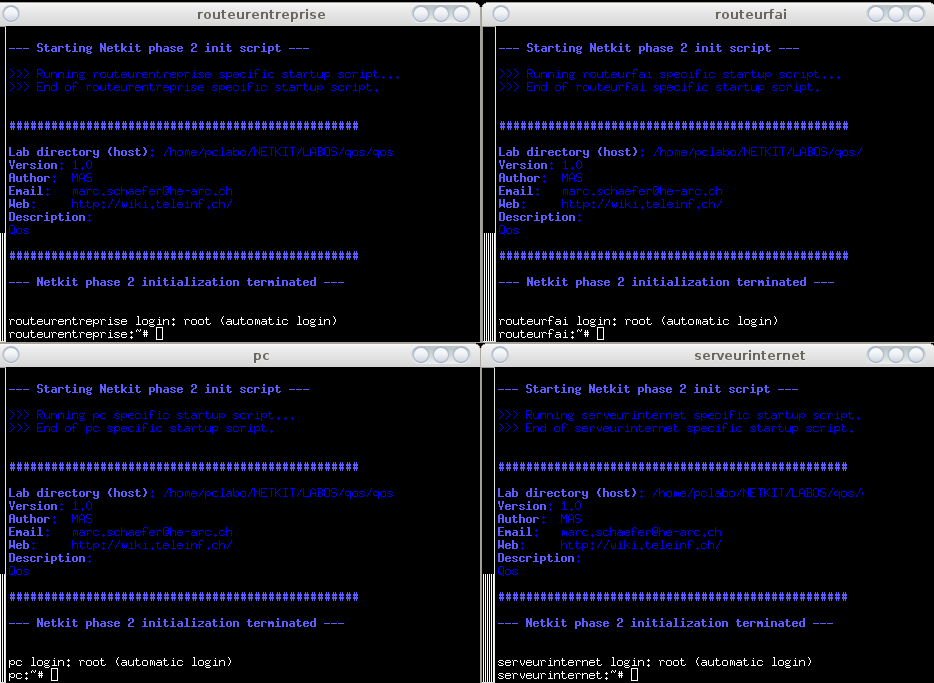
\includegraphics[width=\linewidth]{./captures/1-start.png}
  \caption{Démarrage du labo netkit "QoS"}
  \label{fig:qos}
\end{figure}

Figure \ref{fig:qos} représente le démarrage du laboratoir netkit "qos".

\newpage

\subsection{Traffic Shaping Simple}


\subsection{Marquage du trafic classifié}

\subsection{Classification et traffic shaping hiérarchique}

\subsection{Traffic descendant}

\section{Questions de base}

\subsection*{1 : Expliquer en quelques mots le principe l'algorithme de régulation TCP}

Certains routeur vont marquer les pacquets lorsqu'ils s'apprêtent à subir une congestion, ce système s'appelle l'ECN (Explicit Congestion Notification). Mais ce système mise sur le fait que les d'autres routeurs implément ce système. \cite{cours}

- Certains routeurs lorsqu'ils sont surchargé et s'ils disposent de la fonctionnalité NAGGLE marquent les pacquets par un flag afin de signaler aux clients que leurs messages passent par des zones surchargées.
- Le client va ensuite automatiquement diminuer son débit et le remonter progressivement

\subsection*{2 : Pourquoi un MTU plus faible peut améliorer la QoS?}

- Problème de partage des trames
- Guigge de phase très variable
- Baisse de l'efficacité mais augment le temsp de réponse

\subsection*{3 : Que doit faire un opérateur lorsqu'il remarque des bits TOS et DIFFSERV ?}

Une des 3 possibilités:
- Jeter les pacquets
- ignorer le flag TOS
- supprimer le flag TOS

\subsection*{4 : Pourquoi un MTU plus faible peut améliorer la QoS?}

- Ralentir le débit montant de cette connexion
- Supprimer des paquets de confirmation


\subsection*{5 : Comment diminuer la vitesse du sens descendant en modifiant celle du sens montant?}

- Limiter le nombre de ack par exemple en groupant les confirmations comme go back-n
- Priorisation du traffic montant, confirmations


\subsection*{6 : Pourquoi gérer le traffic shaping seulement sur routeurentreprise produit de bon résultat mais n'est toujours pas suffisant?}

- Routeur entreprise ne peux pas gérer le traffic plus général qui sera plus important sur le routeur FAI.
- Routeur FAI aura un traffic plus important que le routeur entreprise
- Parce que on peut déjà prioriser notre traffic en interne.

\subsection*{7 : Quelle queue est recommendé pour garantir un traitement équitables des données?}

- SFQ (stochastic fair queuing)
- Non car il va jeter ce qui déborde

\section{Questions rapport}

\subsection*{1 : Qu'est ce que le routage de la patate chaude et à quoi sert-il dans un réseau surchargé?}

- Il envoie tout ce qu'il reçoit et s'il y a un routeur qui est surchargé, il envoie le paquet à un autre routeur

\subsection{2 : Avec quel outil peut-on évaluer le nombre de paquets reçus en désordre?}

- Wireshark avec des filtres

\subsection*{3 : Proposer une répartition de débit entre classes plus logique dans un réseau réel}

- Prioriser le tcp

\subsection*{4 : Conception d'un baquet}

%\begin{minted}{python}

%\end{minted}


\section{Conclusion}

\printbibliography

\end{document}
